

\tikzset{every picture/.style={line width=0.75pt}} %set default line width to 0.75pt        

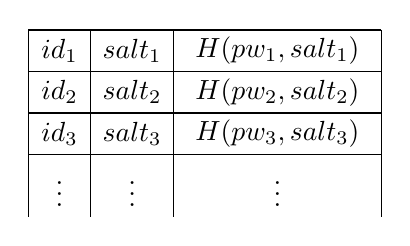
\begin{tikzpicture}[x=0.75pt,y=0.75pt,yscale=-1,xscale=1]
%uncomment if require: \path (0,94); %set diagram left start at 0, and has height of 94

%Straight Lines [id:da48690891710689943] 
\draw  [line width=0.5]  (0,0) -- (0,90) ;
%Straight Lines [id:da07883832722873985] 
\draw  [line width=0.5]  (0,0) -- (170,0) ;
%Straight Lines [id:da39136603292686534] 
\draw  [line width=0.5]  (30,0) -- (30,90) ;
%Straight Lines [id:da18677337990047116] 
\draw  [line width=0.5]  (170,0) -- (170,90) ;
%Straight Lines [id:da7111238231534653] 
\draw  [line width=0.5]  (0,20) -- (170,20) ;
%Straight Lines [id:da28765771561296405] 
\draw  [line width=0.5]  (0,40) -- (170,40) ;
%Straight Lines [id:da41036851267981467] 
\draw  [line width=0.5]  (0,60) -- (170,60) ;
%Straight Lines [id:da9078156775792283] 
\draw  [line width=0.5]  (70,0) -- (70,90) ;

% Text Node
\draw (15,10) node    {$id_{1}$};
% Text Node
\draw (15,30) node    {$id_{2}$};
% Text Node
\draw (15,50) node    {$id_{3}$};
% Text Node
\draw (15,75) node    {$\vdots $};
% Text Node
\draw (120,10) node    {$H( pw_{1} ,salt_{1})$};
% Text Node
\draw (50,75) node    {$\vdots $};
% Text Node
\draw (50,10) node    {$salt_{1}$};
% Text Node
\draw (50,30) node    {$salt_{2}$};
% Text Node
\draw (50,50) node    {$salt_{3}$};
% Text Node
\draw (120,30) node    {$H( pw_{2} ,salt_{2})$};
% Text Node
\draw (120,50) node    {$H( pw_{3} ,salt_{3})$};
% Text Node
\draw (120,75) node    {$\vdots $};


\end{tikzpicture}